
Para ver el rechazo de ruido que presenta la fuente de alimentación, sumamos a la tensión de entrada una señal en forma de diente de sierra descendente de $100 Hz$, ya que la sugerencia era que el ruido podría provenir del rizado resultante de una rectificación y filtrado. Se utilizó una señal de $2 V$ de amplitud para poder apreciar bien la amplitud de la señal en la salida. Se graficó la entrada y la salida restándole la tensión continua de base, $20 V$ a la entrada y el valor mínimo a la salida, alrededor de $2 V$, se utilizó un script de \textbf{MATLAB} para restar los valores adecuados, hacer los cálculos y producir los gráficos a partir de los datos exportados del \textbf{LTSPICE}. En la figura~\figref{fig:fig_p20_ripple}, se muestra lo obtenido, mostrando simultáneamente 2 ciclos del rizado de entrada y salida.
Como se observa en la figura, la salida presenta un cierto tiempo de crecimiento debido al ancho de banda limitado del amplificador de la fuente, y presenta además un pequeño pico en la discontinuidad, el mismo se debe al tipo de compensación del circuito, tema que veremos en la siguiente parte del trabajo práctico. Si se mide el rechazo de ruido simplemente como el cociente de valor RMS de la señal de salida respecto de la entrada obtenemos:


\begin{equation}
    R_{nr}= 59.49 dB
\end{equation}

Sin embargo se pedía intentar no considerar el ruido propio de la fuente, entonces lo que se hizo fue, extrapolar la amplitud máxima de la señal de rizado a la salida, ignorando el sobre-pico y el tiempo de crecimiento, midiendo su amplitud cerca de la mitad de la amplitud máxima de la señal de entrada, calculado así, obtuvimos:


\begin{equation}
    R_{nr}= 61.41 dB
\end{equation}

\vfill

\clearpage

\begin{figure}[H] %htb
\begin{center}
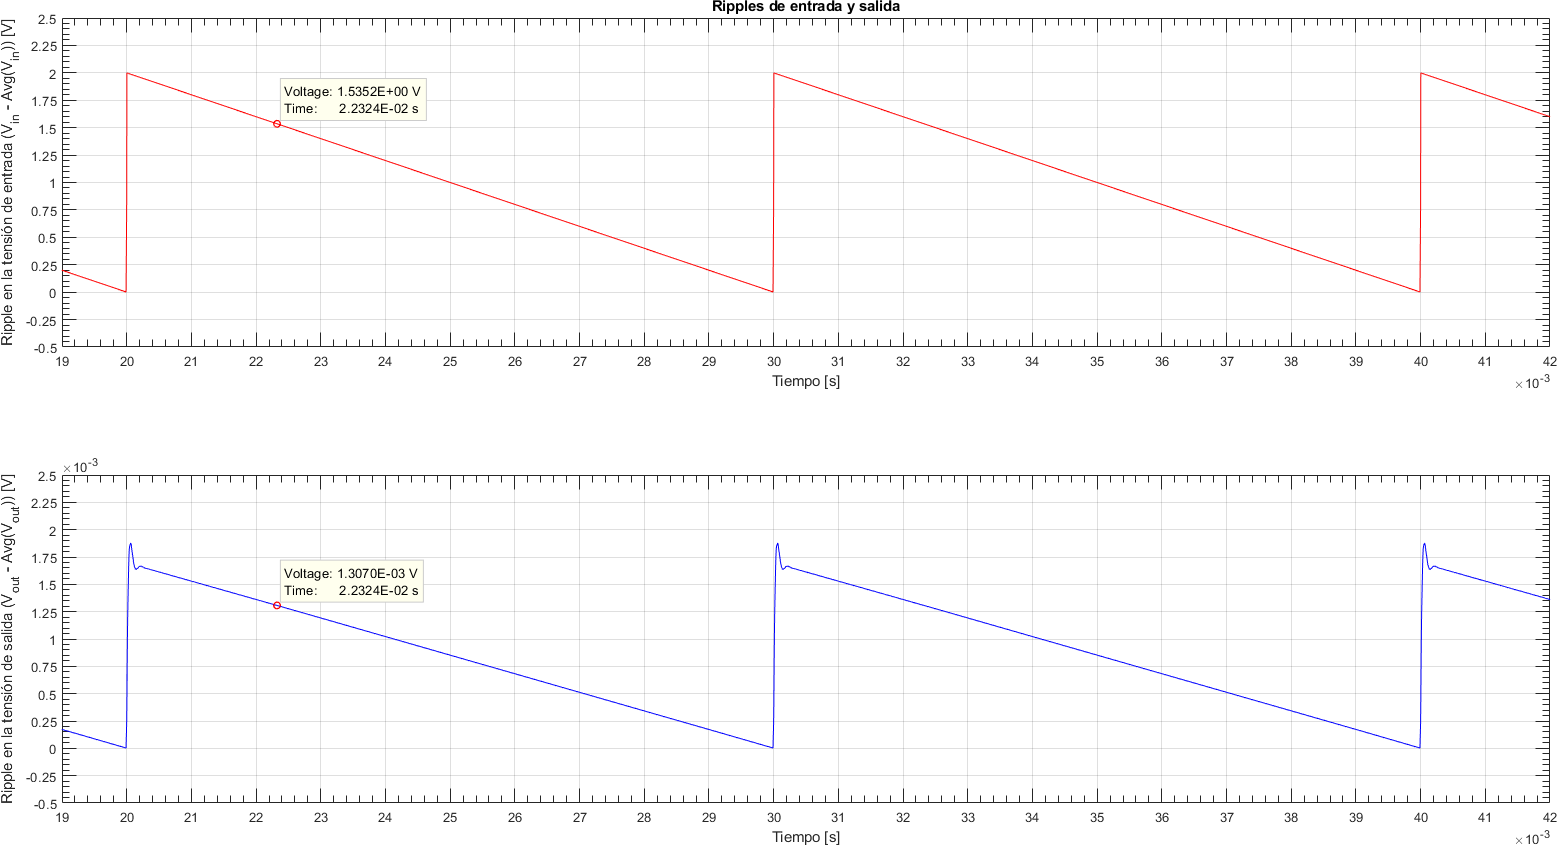
\includegraphics[width=1.2 \textwidth, angle=90]{./img/preguntas/p20.png}
\caption{\label{fig:fig_p20_ripple}\footnotesize{Rizado de entrada y salida.}}
\end{center}
\end{figure}

\clearpage